
\documentclass[letterpaper,hide notes,xcolor={table,svgnames},pdftex,10pt]{beamer}
\def\showexamples{t}

\usecolortheme{crane}
\setbeamertemplate{navigation symbols}{}

\usetheme{MyPittsburgh}
\usepackage{hyperref}
\usepackage{graphicx,xspace}
\usepackage[normalem]{ulem}
\usepackage{multicol}
\usepackage{amsmath,amssymb,amsthm,graphicx,xspace}
\newcommand\SF[1]{$\bigstar$\footnote{SF: #1}}

\usepackage[sfdefault,lf]{carlito}
\usepackage[T1]{fontenc}
\usepackage[scaled]{beramono}
\usepackage{tikzpagenodes}
\newcommand{\Rplus}{\protect\hspace{-.1em}\protect\raisebox{.35ex}{\small{\small\textbf{+}}}}
\newcommand{\Cpp}{\mbox{C\Rplus\Rplus}\xspace}

\newcounter{tmpnumSlide}
\newcounter{tmpnumNote}

\newcommand\mnote[1]{%
	\addtocounter{tmpnumSlide}{1}
	\ifdefined\showcues {~\tiny\fbox{\arabic{tmpnumSlide}}}\fi
	\note{\setlength{\parskip}{1ex}\addtocounter{tmpnumNote}{1}\textbf{\Large \arabic{tmpnumNote}:} {#1\par}}}

\newcommand\mmnote[1]{\note{\setlength{\parskip}{1ex}#1\par}}


\newcommand\mquestion[2]{{~\color{red}\fbox{?}}\note{\setlength{\parskip}{1ex}\par{\Large \textbf{?}} #1} \note{\setlength{\parskip}{1ex}\par{\Large \textbf{A}} #2\par}\ifdefined \presentationonly \pause \fi}

\newcommand\blackboard[1]{%
	\ifdefined   \showblackboard
		{#1}
	\else {\begin{center} \fbox{\colorbox{blue!30}{%
						\begin{minipage}{.95\linewidth}%
							\hspace{\stretch{1}} Some space intentionally left blank; done at the blackboard.%
						\end{minipage}}}\end{center}}%
	\fi%
}

\usepackage{listings}
\lstset{%
	keywordstyle=\bfseries,
	aboveskip=15pt,
	belowskip=15pt,
	captionpos=b,
	identifierstyle=\ttfamily,
	frame=lines,
	numbers=left, basicstyle=\scriptsize, numberstyle=\tiny, stepnumber=0, numbersep=2pt}

\usepackage{siunitx}
\newcommand\sius[1]{\num[group-separator = {,}]{#1}\si{\micro\second}}
\newcommand\sims[1]{\num[group-separator = {,}]{#1}\si{\milli\second}}
\newcommand\sins[1]{\num[group-separator = {,}]{#1}\si{\nano\second}}
\sisetup{group-separator = {,}, group-digits = true}

%% -------------------- tikz --------------------
\usepackage{tikz}
\usetikzlibrary{positioning}
\usetikzlibrary{arrows,backgrounds,automata,decorations.shapes,decorations.pathmorphing,decorations.markings,decorations.text}

\tikzstyle{place}=[circle,draw=blue!50,fill=blue!20,thick, inner sep=0pt,minimum size=6mm]
\tikzstyle{transition}=[rectangle,draw=black!50,fill=black!20,thick, inner sep=0pt,minimum size=4mm]

\tikzstyle{block}=[rectangle,draw=black, thick, inner sep=5pt]
\tikzstyle{bullet}=[circle,draw=black, fill=black, thin, inner sep=2pt]

\tikzstyle{pre}=[<-,shorten <=1pt,>=stealth',semithick]
\tikzstyle{post}=[->,shorten >=1pt,>=stealth',semithick]
\tikzstyle{bi}=[<->,shorten >=1pt,shorten <=1pt, >=stealth',semithick]

\tikzstyle{mut}=[-,>=stealth',semithick]

\tikzstyle{treereset}=[dashed,->, shorten >=1pt,>=stealth',thin]

\usepackage{ifmtarg}
\usepackage{xifthen}
\makeatletter
% new counter to now which frame it is within the sequence
\newcounter{multiframecounter}
% initialize buffer for previously used frame title
\gdef\lastframetitle{\textit{undefined}}
% new environment for a multi-frame
\newenvironment{multiframe}[1][]{%
	\ifthenelse{\isempty{#1}}{%
		% if no frame title was set via optional parameter,
		% only increase sequence counter by 1
		\addtocounter{multiframecounter}{1}%
	}{%
		% new frame title has been provided, thus
		% reset sequence counter to 1 and buffer frame title for later use
		\setcounter{multiframecounter}{1}%
		\gdef\lastframetitle{#1}%
	}%
	% start conventional frame environment and
	% automatically set frame title followed by sequence counter
	\begin{frame}%
		\frametitle{\lastframetitle~{\normalfont(\arabic{multiframecounter})}}%
		}{%
	\end{frame}%
}
\makeatother

\makeatletter
\newdimen\tu@tmpa%
\newdimen\ydiffl%
\newdimen\xdiffl%
\newcommand\ydiff[2]{%
	\coordinate (tmpnamea) at (#1);%
	\coordinate (tmpnameb) at (#2);%
	\pgfextracty{\tu@tmpa}{\pgfpointanchor{tmpnamea}{center}}%
	\pgfextracty{\ydiffl}{\pgfpointanchor{tmpnameb}{center}}%
	\advance\ydiffl by -\tu@tmpa%
}
\newcommand\xdiff[2]{%
	\coordinate (tmpnamea) at (#1);%
	\coordinate (tmpnameb) at (#2);%
	\pgfextractx{\tu@tmpa}{\pgfpointanchor{tmpnamea}{center}}%
	\pgfextractx{\xdiffl}{\pgfpointanchor{tmpnameb}{center}}%
	\advance\xdiffl by -\tu@tmpa%
}
\makeatother
\newcommand{\copyrightbox}[3][r]{%
	\begin{tikzpicture}%
		\node[inner sep=0pt,minimum size=2em](ciimage){#2};
		\usefont{OT1}{phv}{n}{n}\fontsize{4}{4}\selectfont
		\ydiff{ciimage.south}{ciimage.north}
		\xdiff{ciimage.west}{ciimage.east}
		\ifthenelse{\equal{#1}{r}}{%
			\node[inner sep=0pt,right=1ex of ciimage.south east,anchor=north west,rotate=90]%
			{\raggedleft\color{black!50}\parbox{\the\ydiffl}{\raggedright{}#3}};%
		}{%
			\ifthenelse{\equal{#1}{l}}{%
				\node[inner sep=0pt,right=1ex of ciimage.south west,anchor=south west,rotate=90]%
				{\raggedleft\color{black!50}\parbox{\the\ydiffl}{\raggedright{}#3}};%
			}{%
				\node[inner sep=0pt,below=1ex of ciimage.south west,anchor=north west]%
				{\raggedleft\color{black!50}\parbox{\the\xdiffl}{\raggedright{}#3}};%
			}
		}
	\end{tikzpicture}
}


%% --------------------

%\usepackage[excludeor]{everyhook}
%\PushPreHook{par}{\setbox0=\lastbox\llap{MUH}}\box0}

%\vspace*{\stretch{1}

%\setbox0=\lastbox \llap{\textbullet\enskip}\box0}

\setlength{\parskip}{\fill}

\newcommand\noskips{\setlength{\parskip}{1ex}}
\newcommand\doskips{\setlength{\parskip}{\fill}}

\newcommand\xx{\par\vspace*{\stretch{1}}\par}
\newcommand\xxs{\par\vspace*{2ex}\par}
\newcommand\tuple[1]{\langle #1 \rangle}
\newcommand\code[1]{{\sf \footnotesize #1}}
\newcommand\ex[1]{\uline{Example:} \ifdefined \presentationonly \pause \fi
	\ifdefined\showexamples#1\xspace\else{\uline{\hspace*{2cm}}}\fi}

\newcommand\ceil[1]{\lceil #1 \rceil}


\AtBeginSection[]
{
	\begin{frame}
		\frametitle{Outline}
		\tableofcontents[currentsection]
	\end{frame}
}



\pgfdeclarelayer{edgelayer}
\pgfdeclarelayer{nodelayer}
\pgfsetlayers{edgelayer,nodelayer,main}

\tikzstyle{none}=[inner sep=0pt]
\tikzstyle{rn}=[circle,fill=Red,draw=Black,line width=0.8 pt]
\tikzstyle{gn}=[circle,fill=Lime,draw=Black,line width=0.8 pt]
\tikzstyle{yn}=[circle,fill=Yellow,draw=Black,line width=0.8 pt]
\tikzstyle{empty}=[circle,fill=White,draw=Black]
\tikzstyle{bw} = [rectangle, draw, fill=blue!20,
text width=4em, text centered, rounded corners, minimum height=2em]

\newcommand{\CcNote}[1]{% longname
	This work is licensed under the \textit{Creative Commons #1 3.0 License}.%
}
\newcommand{\CcImageBy}[1]{%
	\includegraphics[scale=#1]{creative_commons/cc_by_30.pdf}%
}
\newcommand{\CcImageSa}[1]{%
	\includegraphics[scale=#1]{creative_commons/cc_sa_30.pdf}%
}
\newcommand{\CcImageNc}[1]{%
	\includegraphics[scale=#1]{creative_commons/cc_nc_30.pdf}%
}
\newcommand{\CcGroupBySa}[2]{% zoom, gap
	\CcImageBy{#1}\hspace*{#2}\CcImageNc{#1}\hspace*{#2}\CcImageSa{#1}%
}
\newcommand{\CcLongnameByNcSa}{Attribution-NonCommercial-ShareAlike}

\newenvironment{changemargin}[1]{% 
	\begin{list}{}{% 
		\setlength{\topsep}{0pt}% 
		\setlength{\leftmargin}{#1}% 
		\setlength{\rightmargin}{1em}
		\setlength{\listparindent}{\parindent}% 
		\setlength{\itemindent}{\parindent}% 
		      \setlength{\parsep}{\parskip}% 
		      }% 
		\item[]}{\end{list}}




\title{Lecture 3 --- Sunrise to Sunset }

\author{Jeff Zarnett \\ \small \texttt{jzarnett@uwaterloo.ca}}
\institute{Department of Electrical and Computer Engineering \\
  University of Waterloo}
\date{\today}


\begin{document}

\begin{frame}
  \titlepage

 \end{frame}

\begin{frame}
\frametitle{Sunrise, Sunset}

\begin{center}
	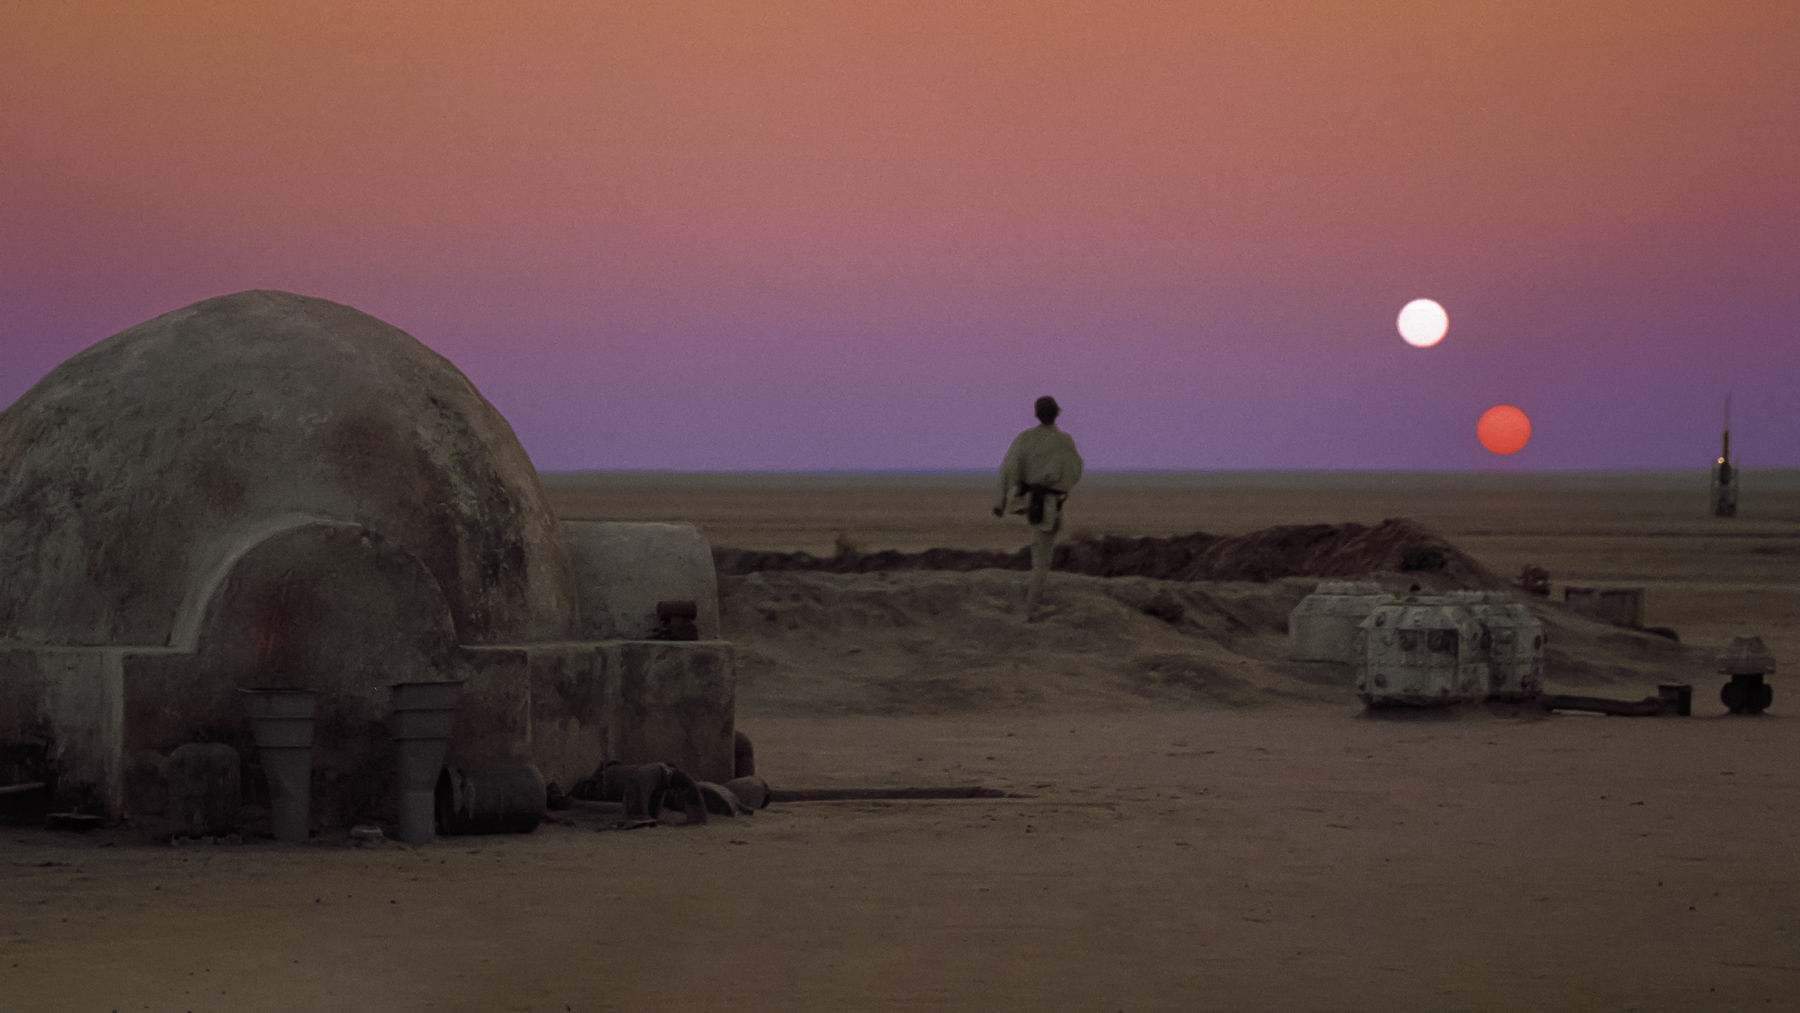
\includegraphics[width=0.9\textwidth]{images/binary_sunset.jpg}
\end{center}


\end{frame}

\begin{frame}
\frametitle{Operating System Lifetime}
We talked about the lifecycle of a process, but an OS has one too!

It is started, executes, and eventually shuts down.

\end{frame}

\begin{frame}
\frametitle{Start Me Up}

Let's imagine the operating system is already installed.

\begin{center}
	
\includegraphics[width=0.7\textwidth]{images/itbegins.jpg}
\end{center}

System startup begins with the BIOS or UEFI.

\end{frame}

\begin{frame}
\frametitle{Boot Loader}

The BIOS or UEFI starts the boot loader.

The boot loader is a small piece of code to start the OS.

It can do some other things.

\end{frame}

\begin{frame}
\frametitle{Start Here}

The boot loader itself has at least some initialization code located in the first block of the hard drive that is the boot device.

\begin{center}
	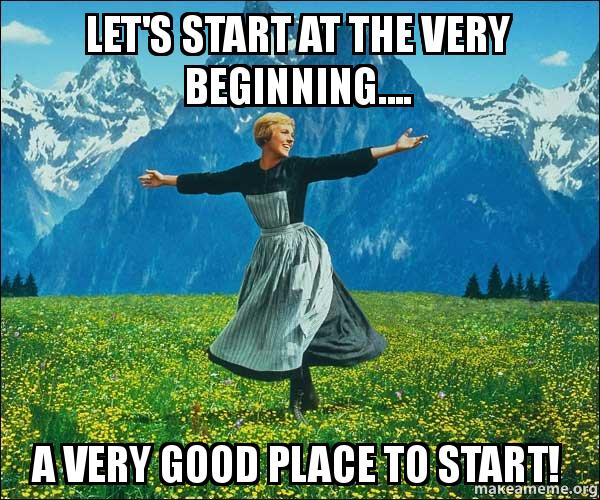
\includegraphics[width=0.4\textwidth]{images/start-beginning.jpg}
\end{center}

Only if the first block of the drive contains this information can it be used for booting.

\end{frame}

\begin{frame}
\frametitle{Kernel Start}

Once the kernel is running, it can start the relevant operating system services.

Some services and utilities are always started when the OS begins running; others are configurable.

Although they are started by the OS without any direct user interaction, most processes are still user-level programs that operate like normal.

\end{frame}

\begin{frame}
\frametitle{By Your Command}

\begin{center}
	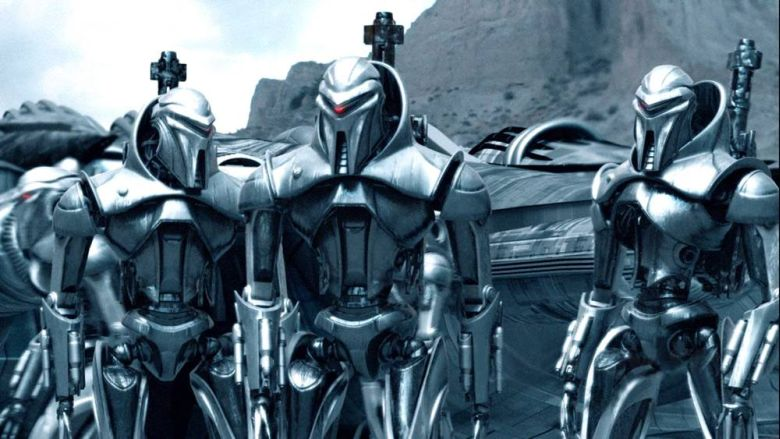
\includegraphics[width=0.6\textwidth]{images/centurions.jpg}
\end{center}
\hfill``By your command.''

The main purpose of the operating system is not to run itself, but is there to make things work for the user-level programs that are supposed to run. 

\end{frame}

\begin{frame}
\frametitle{What Have the Romans Ever Done For Us?}

Some examples of things we already asked the OS to do for us:

\begin{itemize}
	\item Process and thread creation, termination
	\item Inter-process communication
	\item Concurrency control
	\item Memory allocation
\end{itemize}

\end{frame}

\begin{frame}
\frametitle{When You See It...}

The operating system does a lot more than this, and the visibility of that functionality varies.

The OS must check permissions whenever you want to open a file, but you probably do not notice or think about it unless somehow permission is denied.

Scheduling?

\end{frame}

\begin{frame}
\frametitle{OS Structure}

\begin{center}
	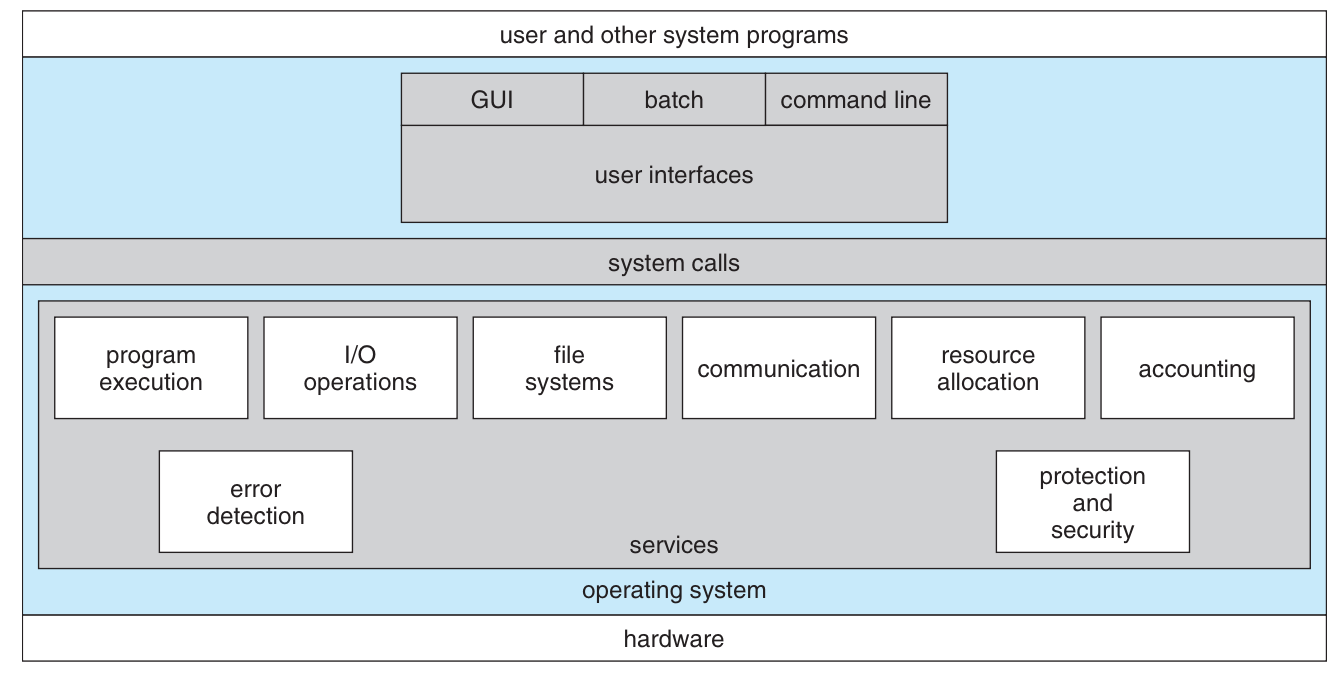
\includegraphics[width=0.75\textwidth]{images/os-structure.png}
\end{center}

\end{frame}

\begin{frame}
\frametitle{Steady-State and Trap}
At steady-state, the operating system runs whatever background tasks it needs to do.

The interesting things happen as the result of a user-level program asking for the OS to do something. 

And you know how that works...

\end{frame}

\begin{frame}
\frametitle{Of Course You Do}

\begin{center}
	
\includegraphics[width=0.65\textwidth]{images/trap2.jpg}
\end{center}

We've covered this from the user-program point of view.

\end{frame}

\begin{frame}
\frametitle{Mode Bits}

We also talked about user mode \& supervisor mode instructions...

Mode bits for the CPU...

Why the I/O operations are managed by the kernel...


\end{frame}

\begin{frame}
\frametitle{Trap Operation}

\begin{center}
	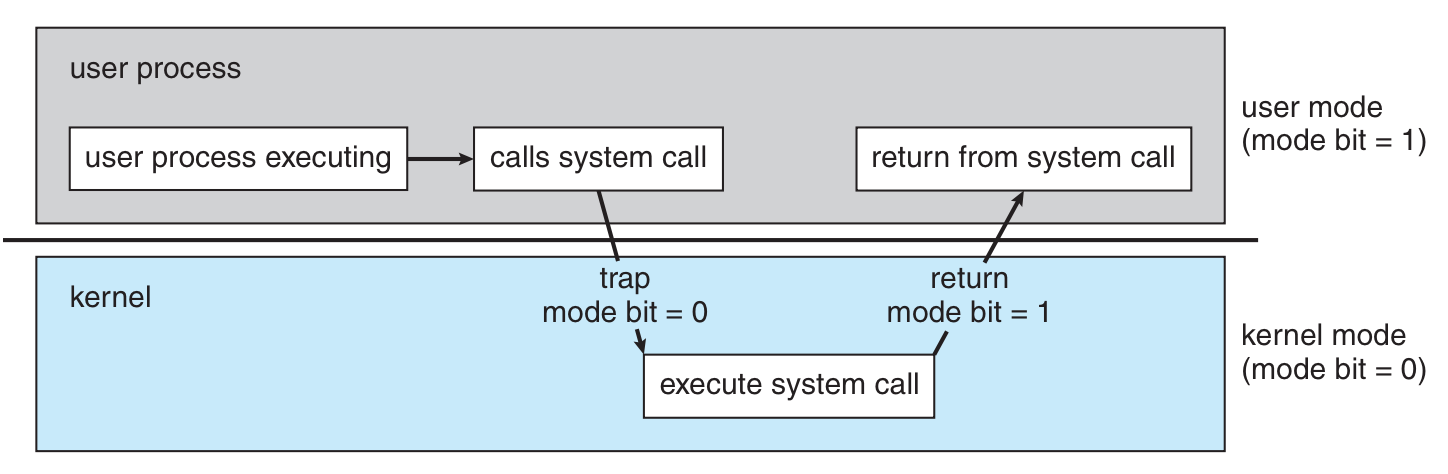
\includegraphics[width=0.75\textwidth]{images/trap.png}\\
	Transition from user to supervisor (kernel) mode~\cite{osc}.
\end{center}


\end{frame}

\begin{frame}
	\frametitle{User Mode and Kernel Mode: Motivation}


	Thanks Uncle Ben: ``with great power comes great responsibility''.


	Same as why we have user accounts and administrator accounts.

	To protect the system \& its integrity against errant and malicious users.


\end{frame}

\begin{frame}
	\frametitle{User Mode and Kernel Mode: Motivation}

	Multiple programs might be trying to use the same I/O device at once.

	Program~1 tries to read from disk. This takes some time.

	If Program~2 wants to read from the same disk, the operating system forces Program~2 to wait its turn.

	Without the OS, it would be up to the author(s) of Program~2 to check and wait patiently for it to become available.

	Works if everyone plays nicely.

	Without enforcement of the rules, a program will do something nasty.

\end{frame}

\begin{frame}
	\frametitle{User Mode and Kernel Mode: Motivation}

	There is a definite performance trade-off.

	Switching from user to kernel mode takes time.

	The performance hit is worth it for the security.

\end{frame}


\begin{frame}
\frametitle{Policy and Mechanism}

\begin{center}
	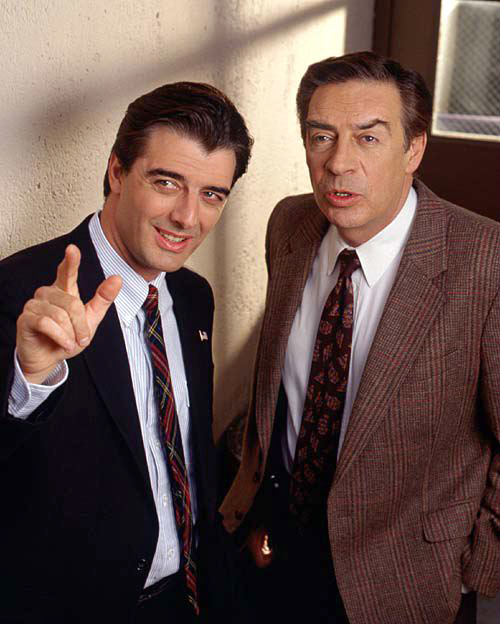
\includegraphics[width=0.35\textwidth]{images/briscoe-logan.jpg}
	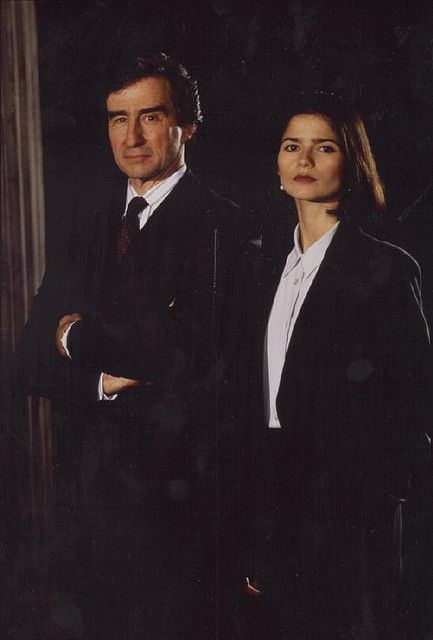
\includegraphics[width=0.35\textwidth]{images/mccoy-kincaid.jpg}
\end{center}

Policy: What will be done.

Mechanism: How policy is carried out.

\end{frame}

\begin{frame}
\frametitle{Policy}
Some policies are configurable:\\
\quad Yes: How much do priorities matter?\\
\quad: No: Can I read from files where I lack the permission?

What is configurable is a question of OS design!

\end{frame}

\begin{frame}
\frametitle{Acropalypse Now}

Applying the policy involves both design and implementation.

OSes err on the side of fewer options.

Do OS authors know best?

\end{frame}

\begin{frame}
\frametitle{Eat Your Vegetables}

From the point of view of the user program, policy is something that we have to contend with but may not have any say in it.

Having to follow the rules may be less convenient, but it's not optional.

The operating system code itself has no such restrictions!

The operating system also has to be responsible for the mechanism.

\end{frame}

\begin{frame}
\frametitle{Switching Time}

Previously: how a switch occurs. Now: when (why)?

From the point of view of the application program we say that the process switch could happen at any time.

The OS does get to choose but it's not a trivial decision.

\end{frame}

\begin{frame}
\frametitle{Interrupt}

\begin{center}
	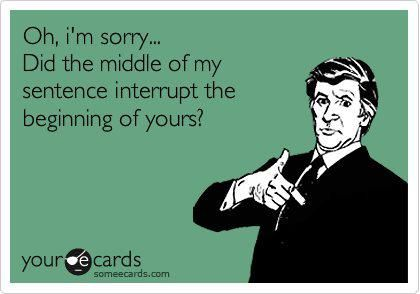
\includegraphics[width=0.5\textwidth]{images/interrupt.jpg}
\end{center}

Interrupt always pauses a thread; may result in a thread switch.


\end{frame}

\begin{frame}
\frametitle{Just Briefly}

A thread switch must occur when the currently-executing one gets blocked.

\begin{center}
	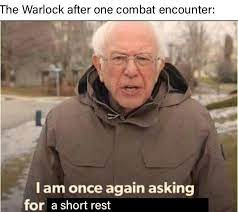
\includegraphics[width=0.4\textwidth]{images/shortrest.jpg}
\end{center}

... or if it terminates.

\end{frame}

\begin{frame}
\frametitle{OS Decision}
After dealing with an interrupt we can choose a new thread.

We also want to prevent monopolization of the CPU...\\
\quad Timer interrupts perhaps?

\end{frame}

\begin{frame}
\frametitle{Take Detailed Notes}

The operating system will have to keep track of the various resources.

\begin{itemize}
	\item Memory Tables
	\item I/O Tables
	\item File Tables
\end{itemize}

\end{frame}

\begin{frame}
\frametitle{Memory Tables}

Track the state of memory: what's free and what's not?

What is the OS memory?

Is any memory shared?

When do we update them?

\end{frame}

\begin{frame}
\frametitle{I/O Tables}
Keep track of the state of I/O devices.

Pay attention to what operations are in progress...

\end{frame}

\begin{frame}
\frametitle{File Tables}

Keep track of which files are open -- process and system level.

Remember -- everything in UNIX is a file!

\end{frame}

\begin{frame}
\frametitle{Power Down}

\begin{center}
	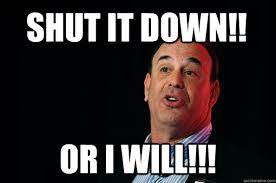
\includegraphics[width=0.4\textwidth]{images/taffer.jpg}
\end{center}

Notify all the running processes they should exit.

\end{frame}

\begin{frame}
\frametitle{But Will They?}

Asking programs to shut down politely may not actually get them to terminate.

\begin{center}
	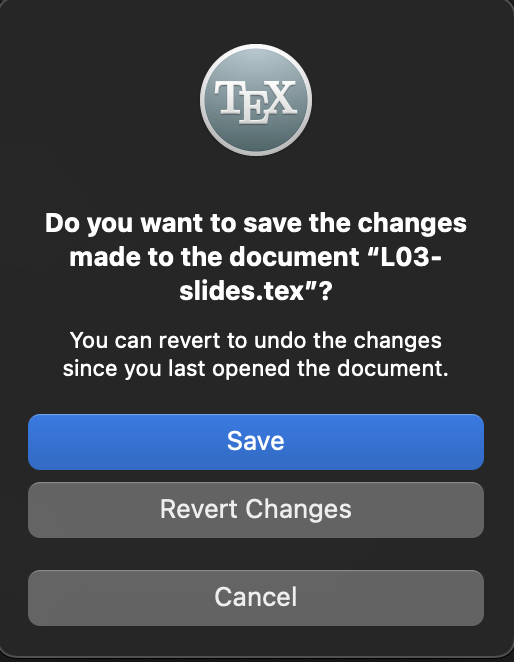
\includegraphics[width=0.4\textwidth]{images/savework.png}
\end{center}

How long do we wait?

\end{frame}

\begin{frame}
\frametitle{Can We Do This?}

Can every user call a shutdown?

Once all processes are done, the OS can terminate its services.

And that's it, power off (or restart).

\end{frame}


\end{document}

